\message{ !name(masters.tex)}\documentclass[]{spie}  %>>> use for US letter paper

\usepackage{graphicx}
\usepackage{subfig}
\usepackage{amsmath}
\usepackage{amssymb}
\usepackage{hyperref}
\usepackage{float}
\usepackage{multirow}

\title{Texture Mapping 3D Models of Indoor Environments with Noisy Camera Poses} 

\author{Peter Cheng
\skiplinehalf
University of California, Berkeley\\
}

\begin{document}

\message{ !name(masters.tex) !offset(938) }
\subsection{Examples}
\label{sec:examples}
As mentioned in Section \ref{sec:dataAcquisition}, the texture mapping
procedure in this thesis can be applied both to low-resolution and
high-resolution models. Low resolution models have an advantage in
their simplicity, and in that only important environmental features
are represented. As a result, images are generated for large sections
of buildings, and boundaries between each texture are minimally
visible. High resolution models have an obvious advantage in terms of
the amount of detail that can be reconstructed, but with poor region
partitioning, as described in Section \ref{sec:geometryPartitioning},
or with high camera pose or geometry reconstruction error, 3D elements
in the environment geometry may not match up well with their imaged
counterparts.

\begin{figure}
  \centering
  \subfloat[][]{
    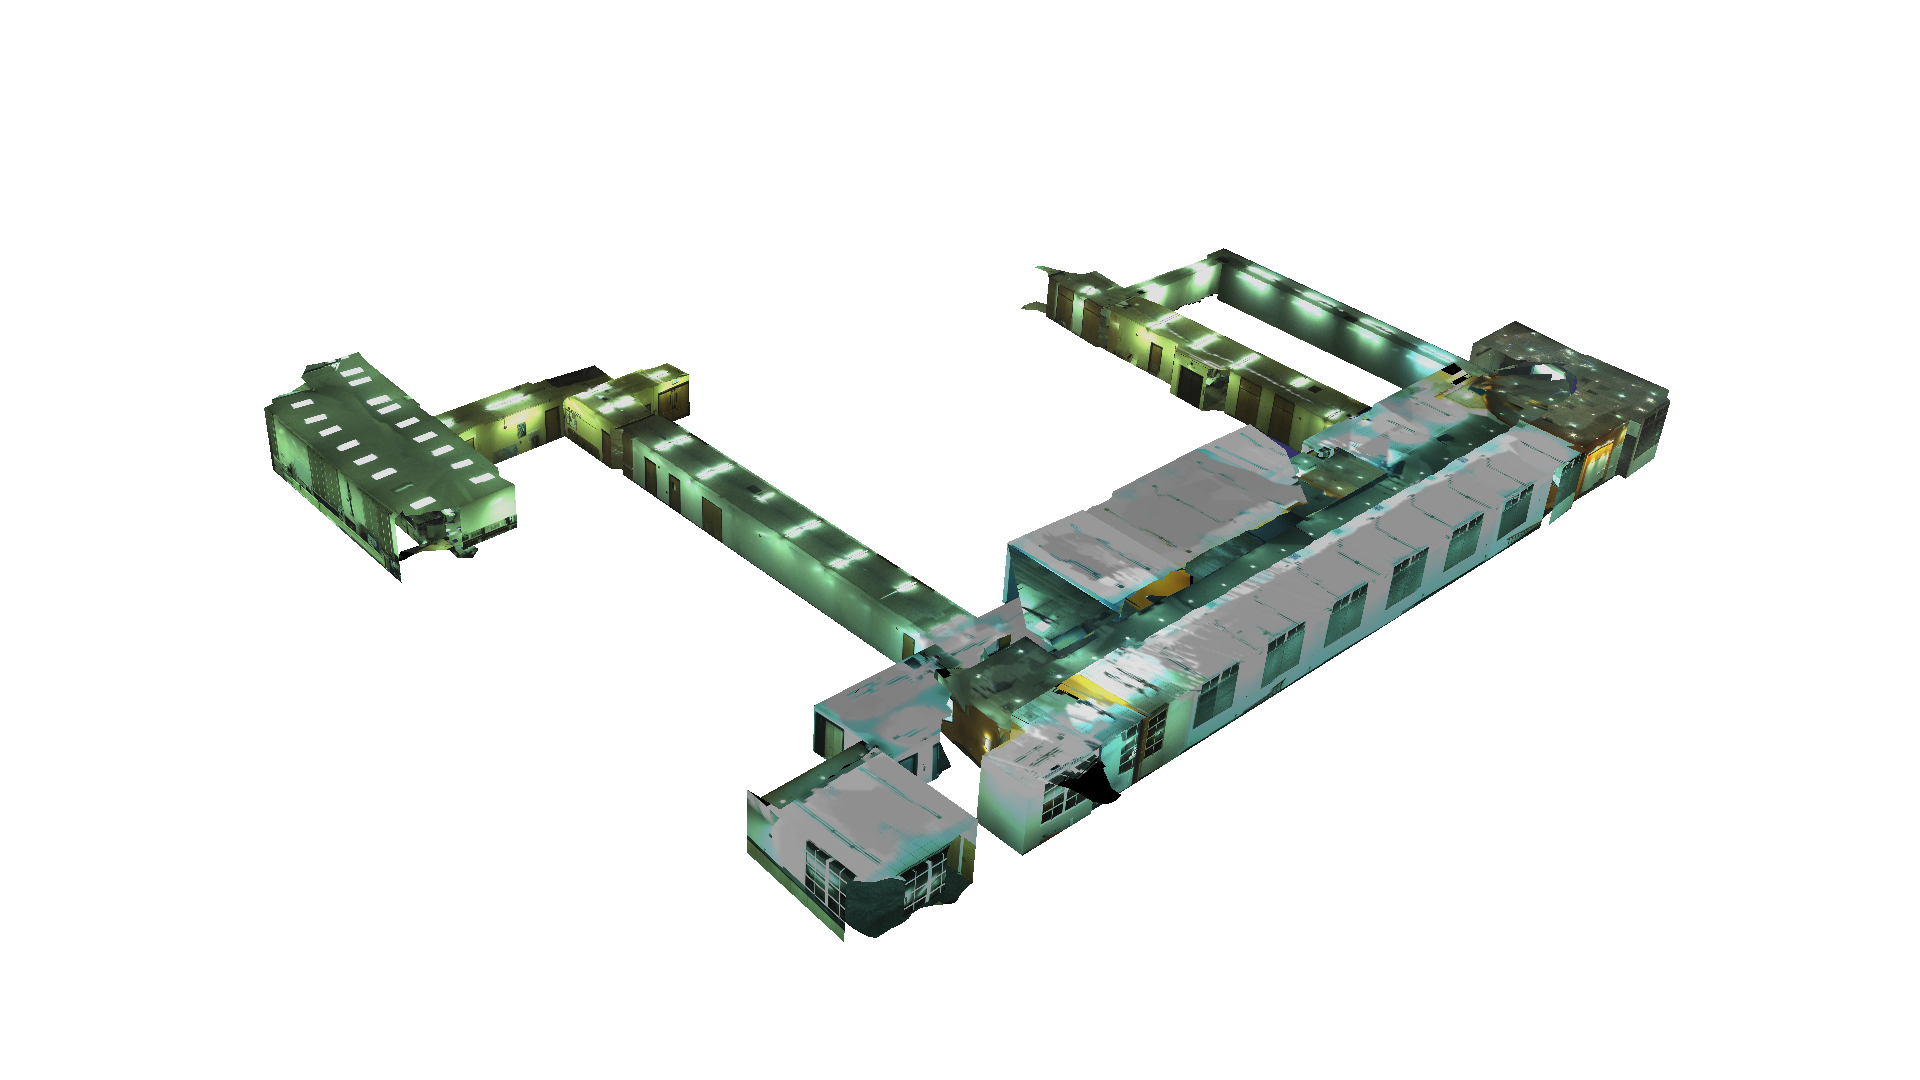
\includegraphics[width=2in]{results_swarm_3_v.jpg}
    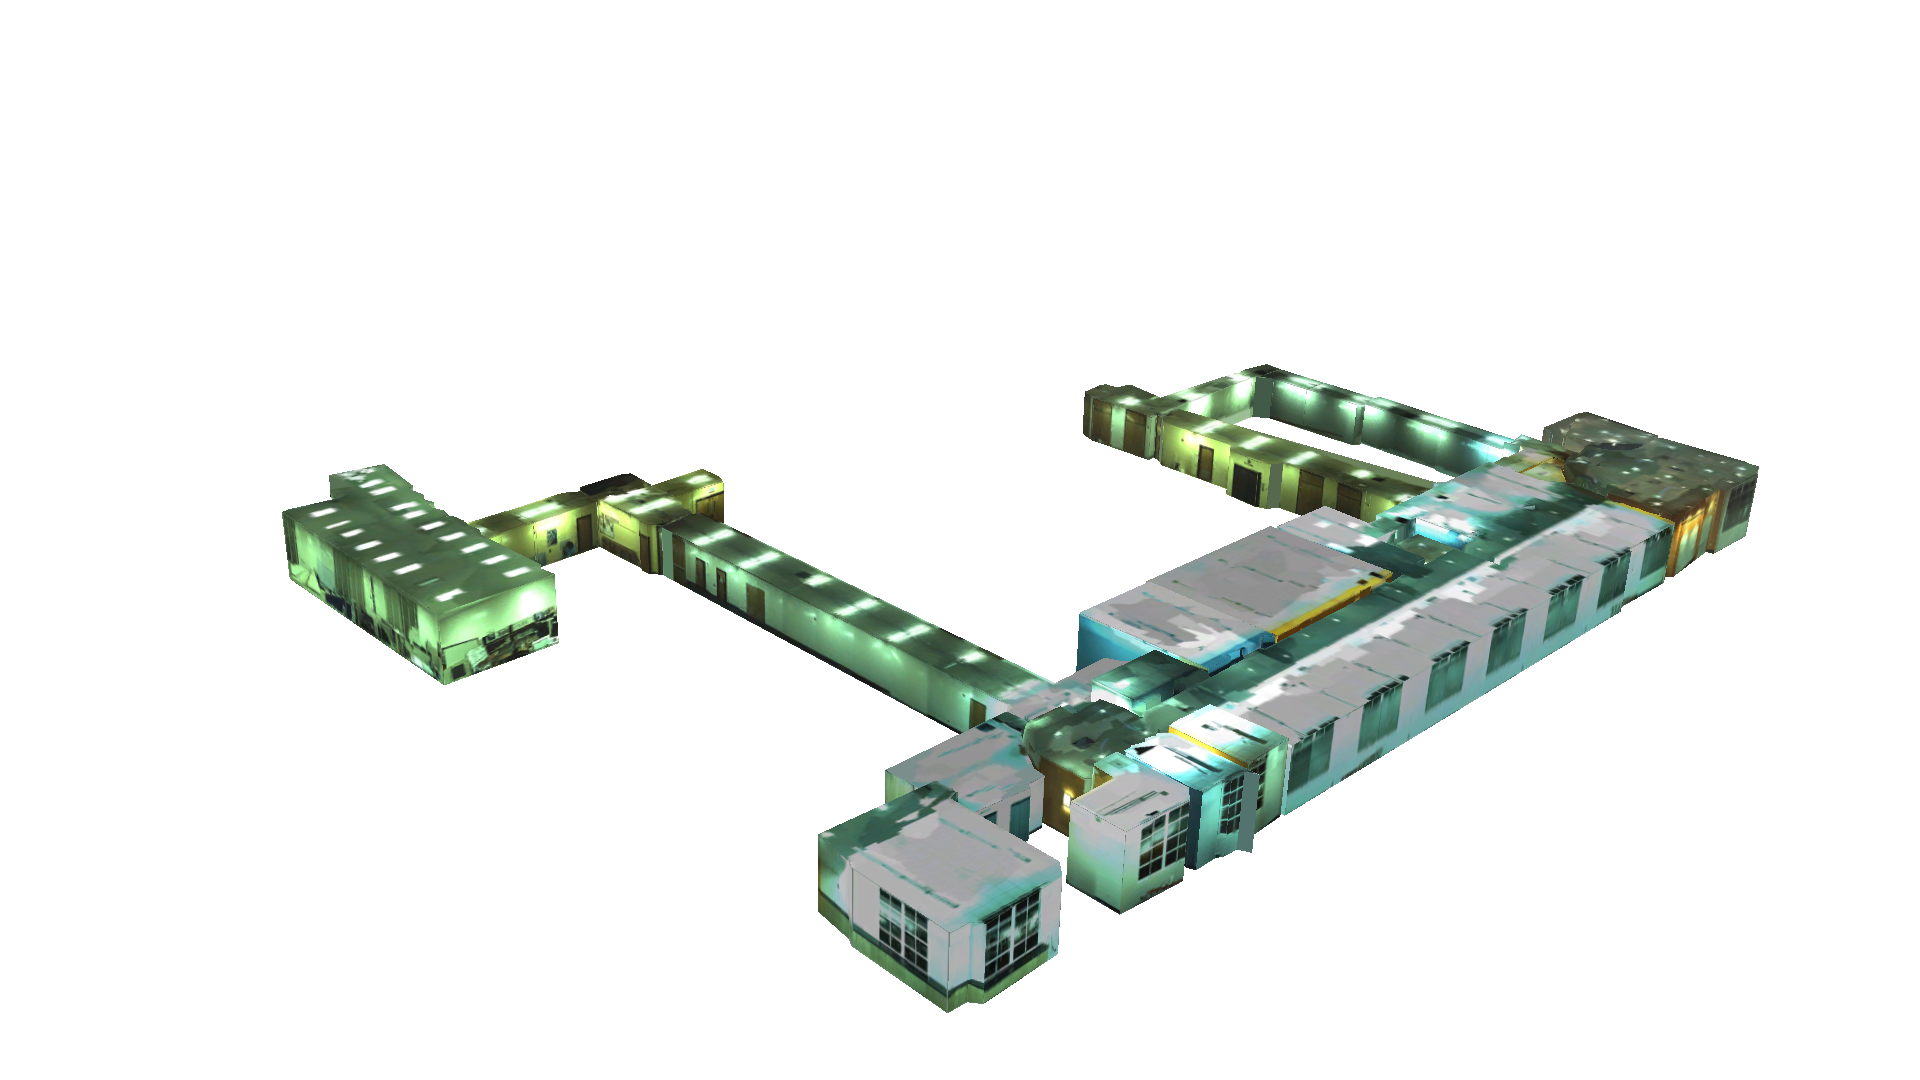
\includegraphics[width=2in]{results_swarm_3_2d.jpg}
    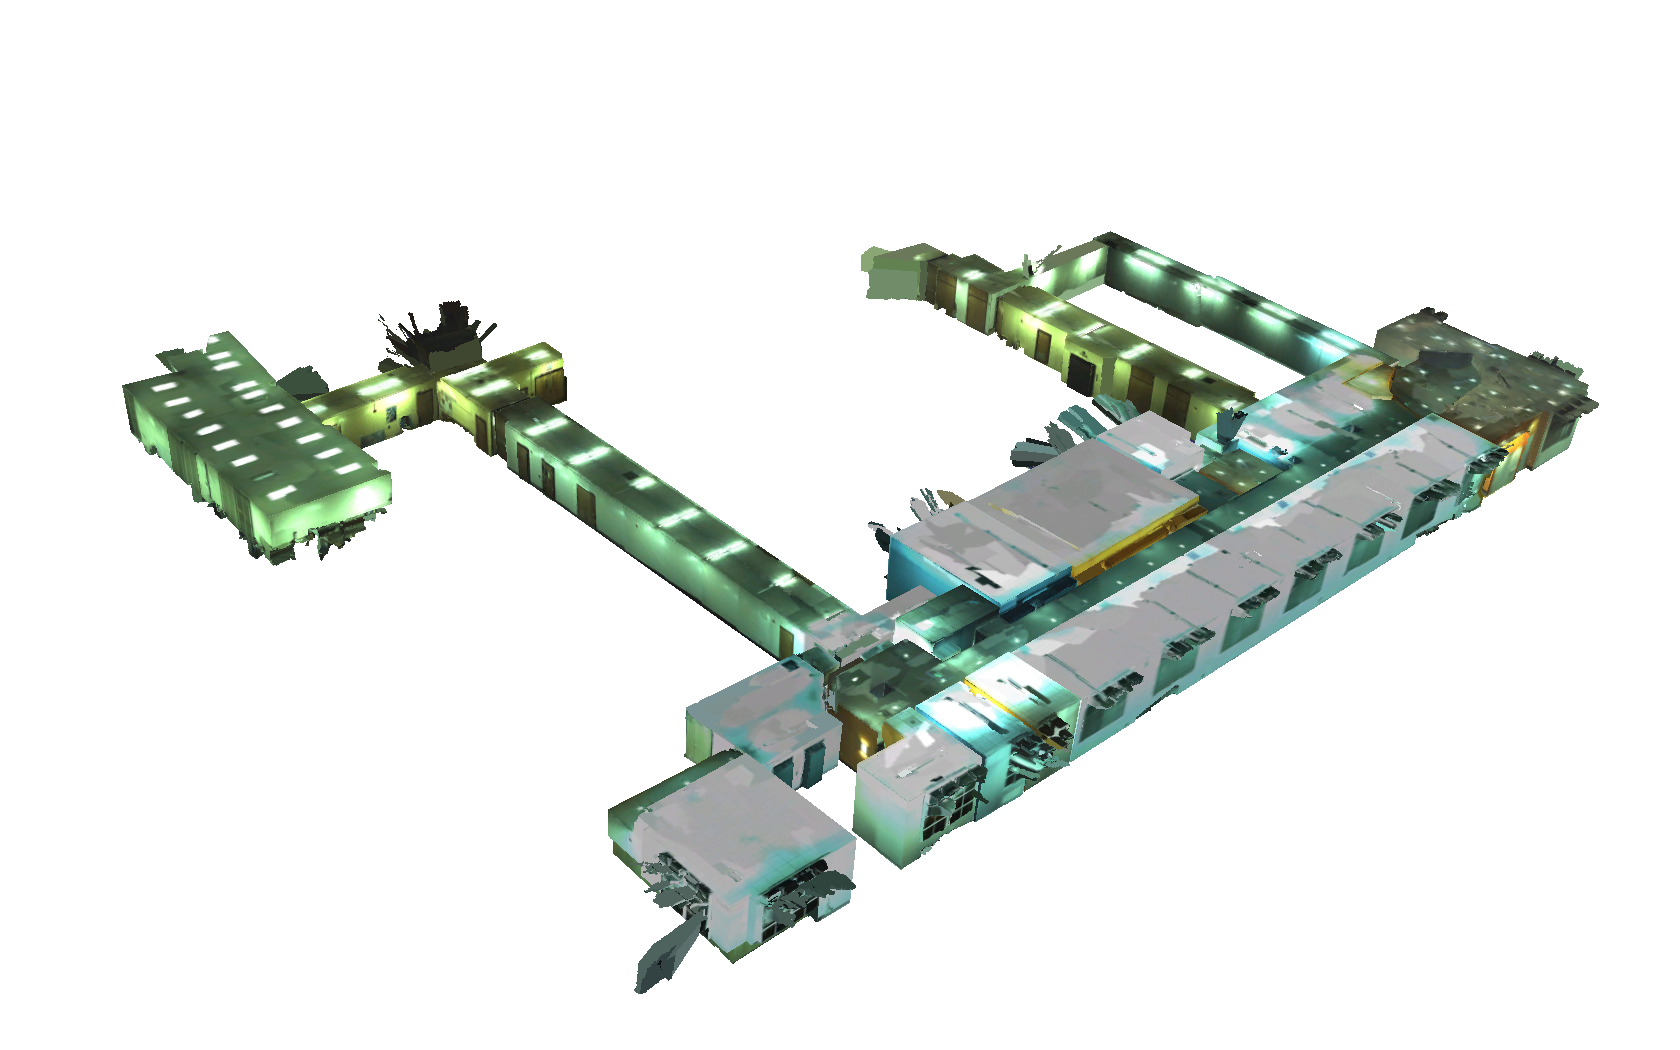
\includegraphics[width=2in]{results_swarm_3_3d.jpg}
  }
  \subfloat[][]{
    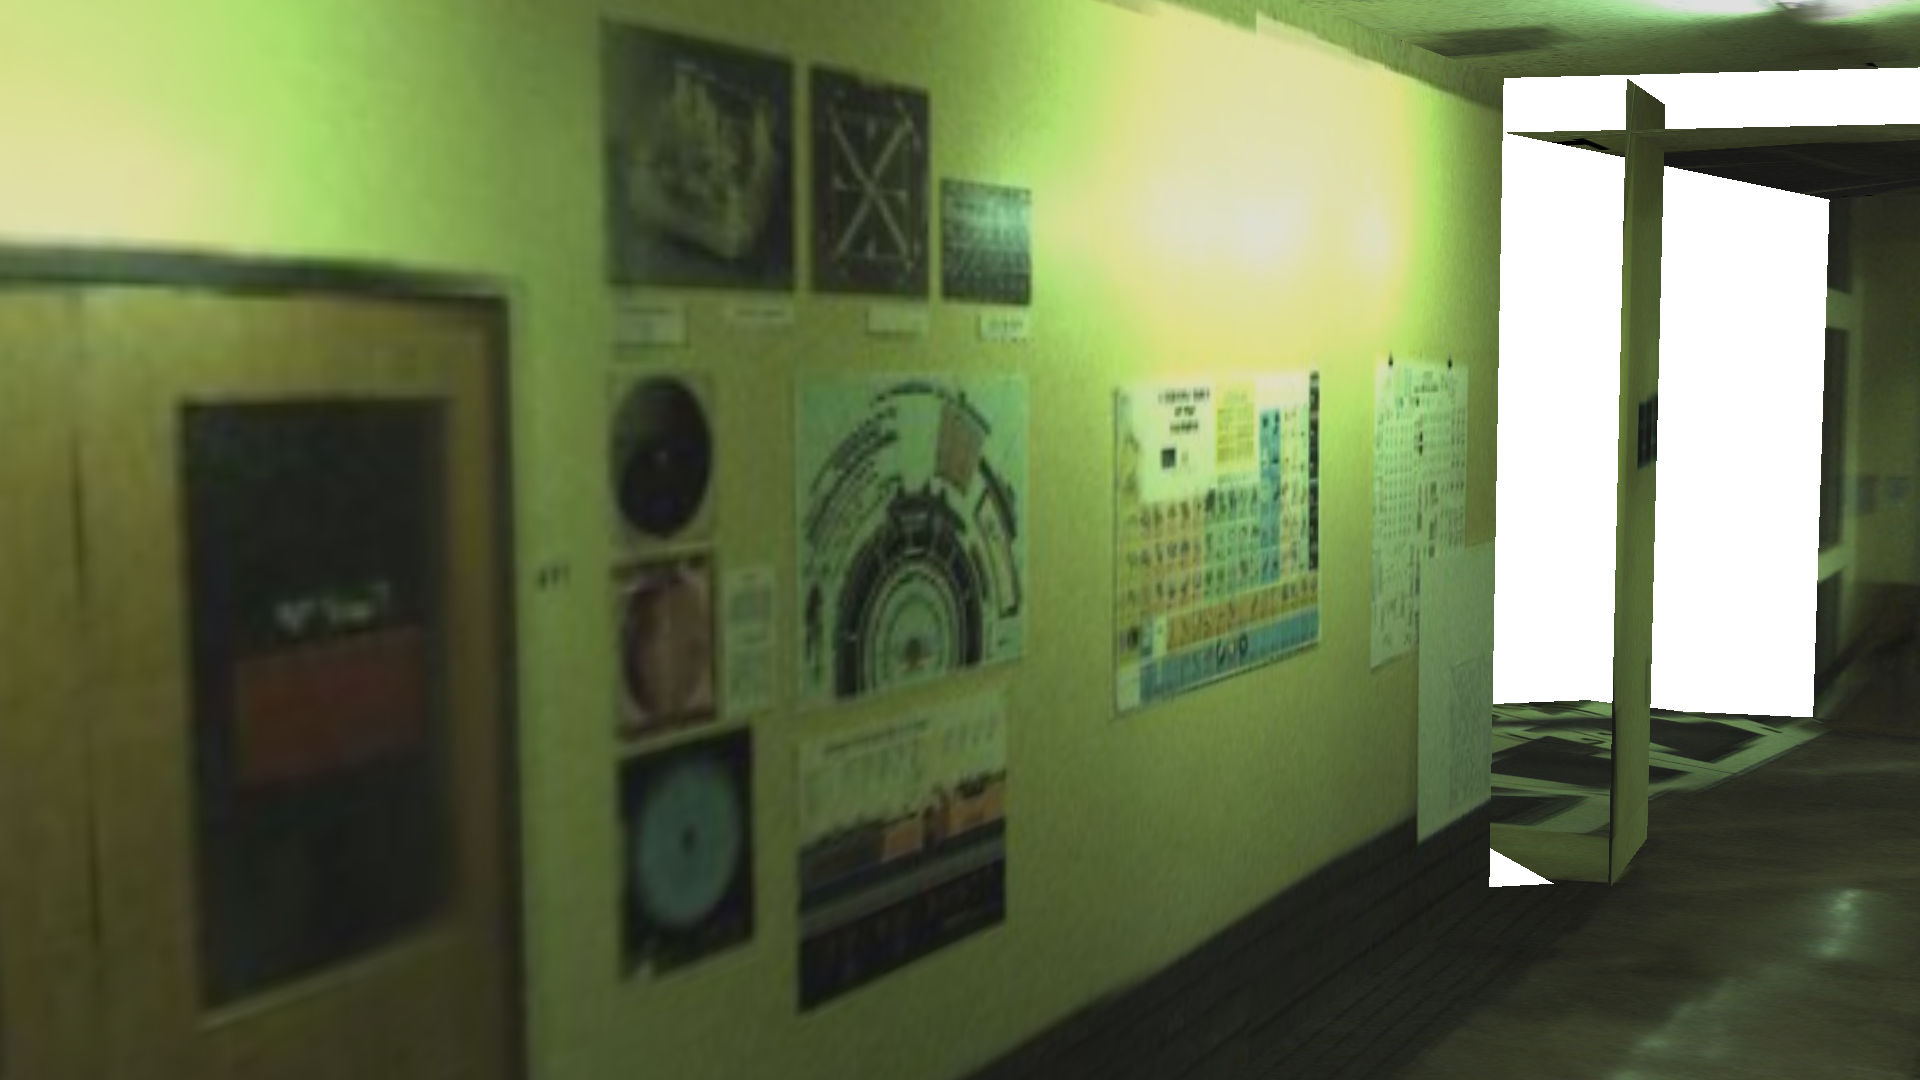
\includegraphics[width=2in]{results_swarm_2_v.jpg}
    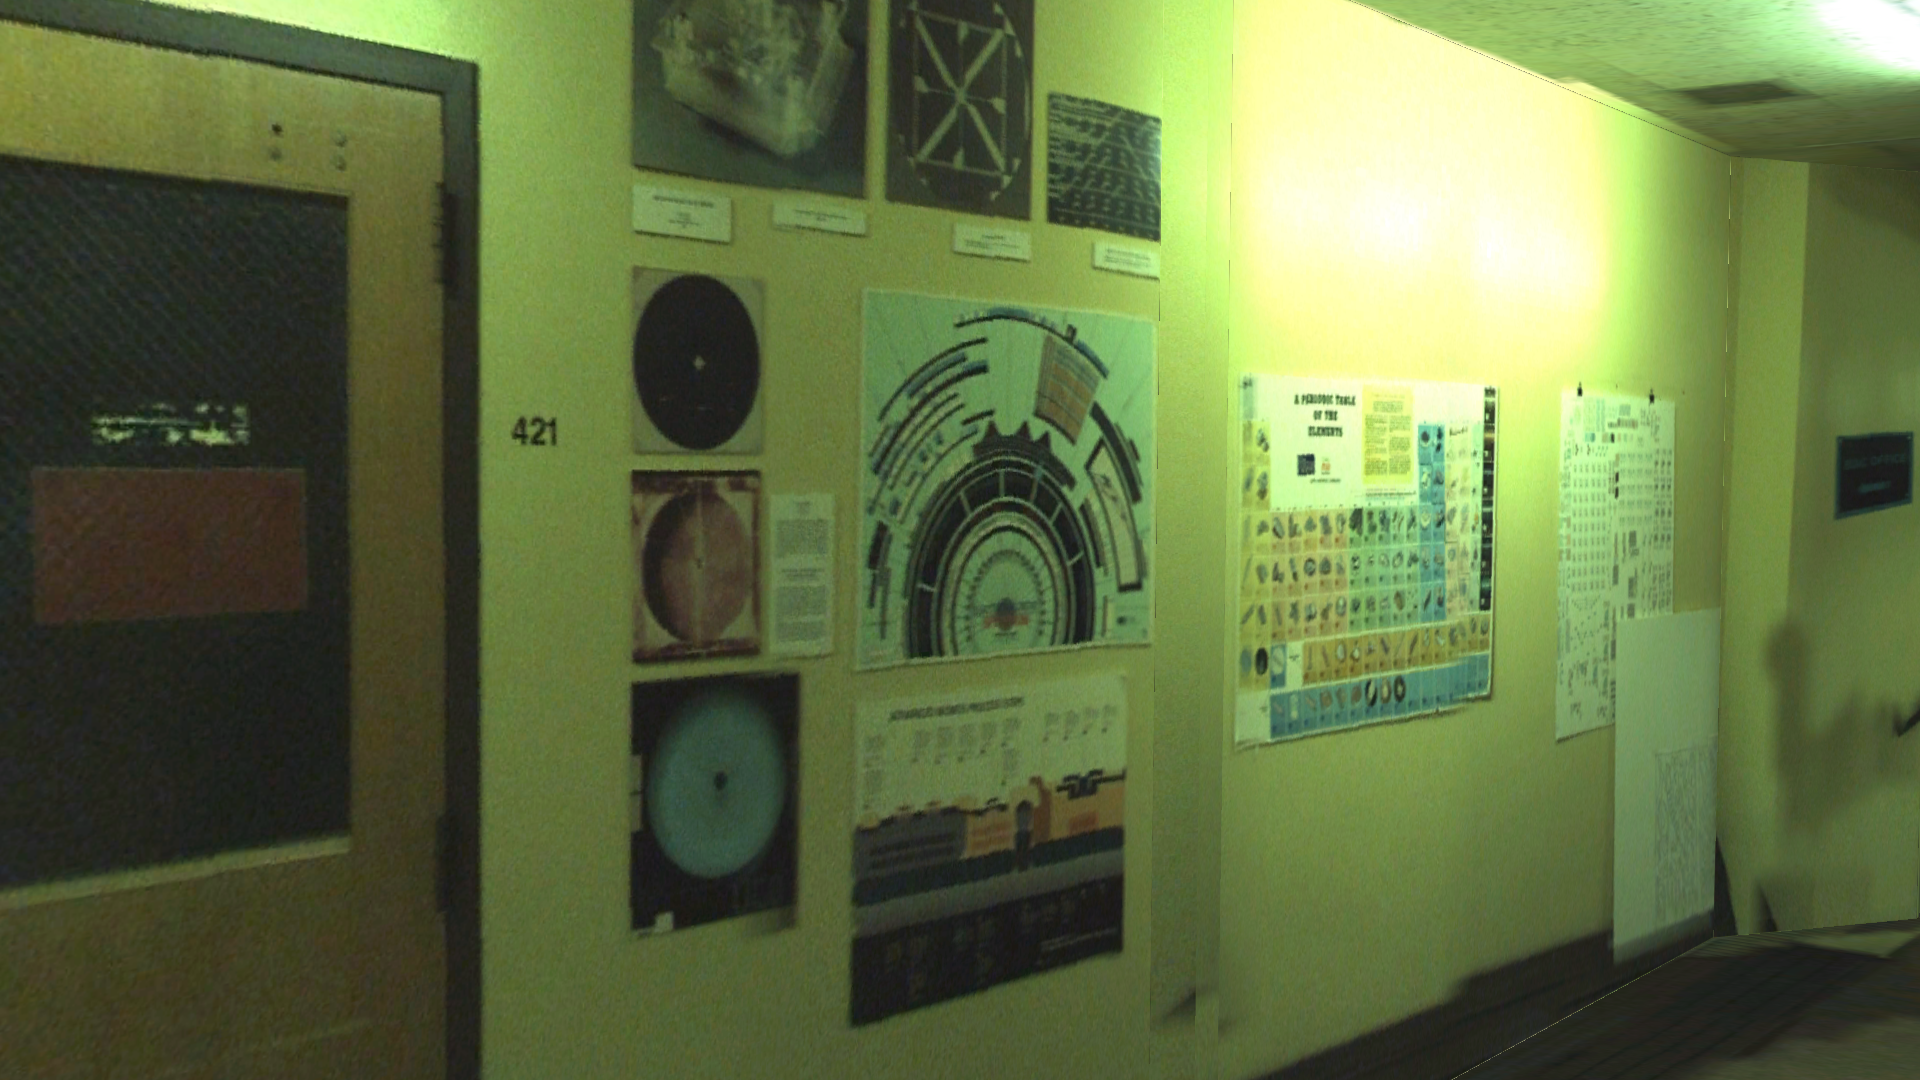
\includegraphics[width=2in]{results_swarm_2_2d.jpg}
    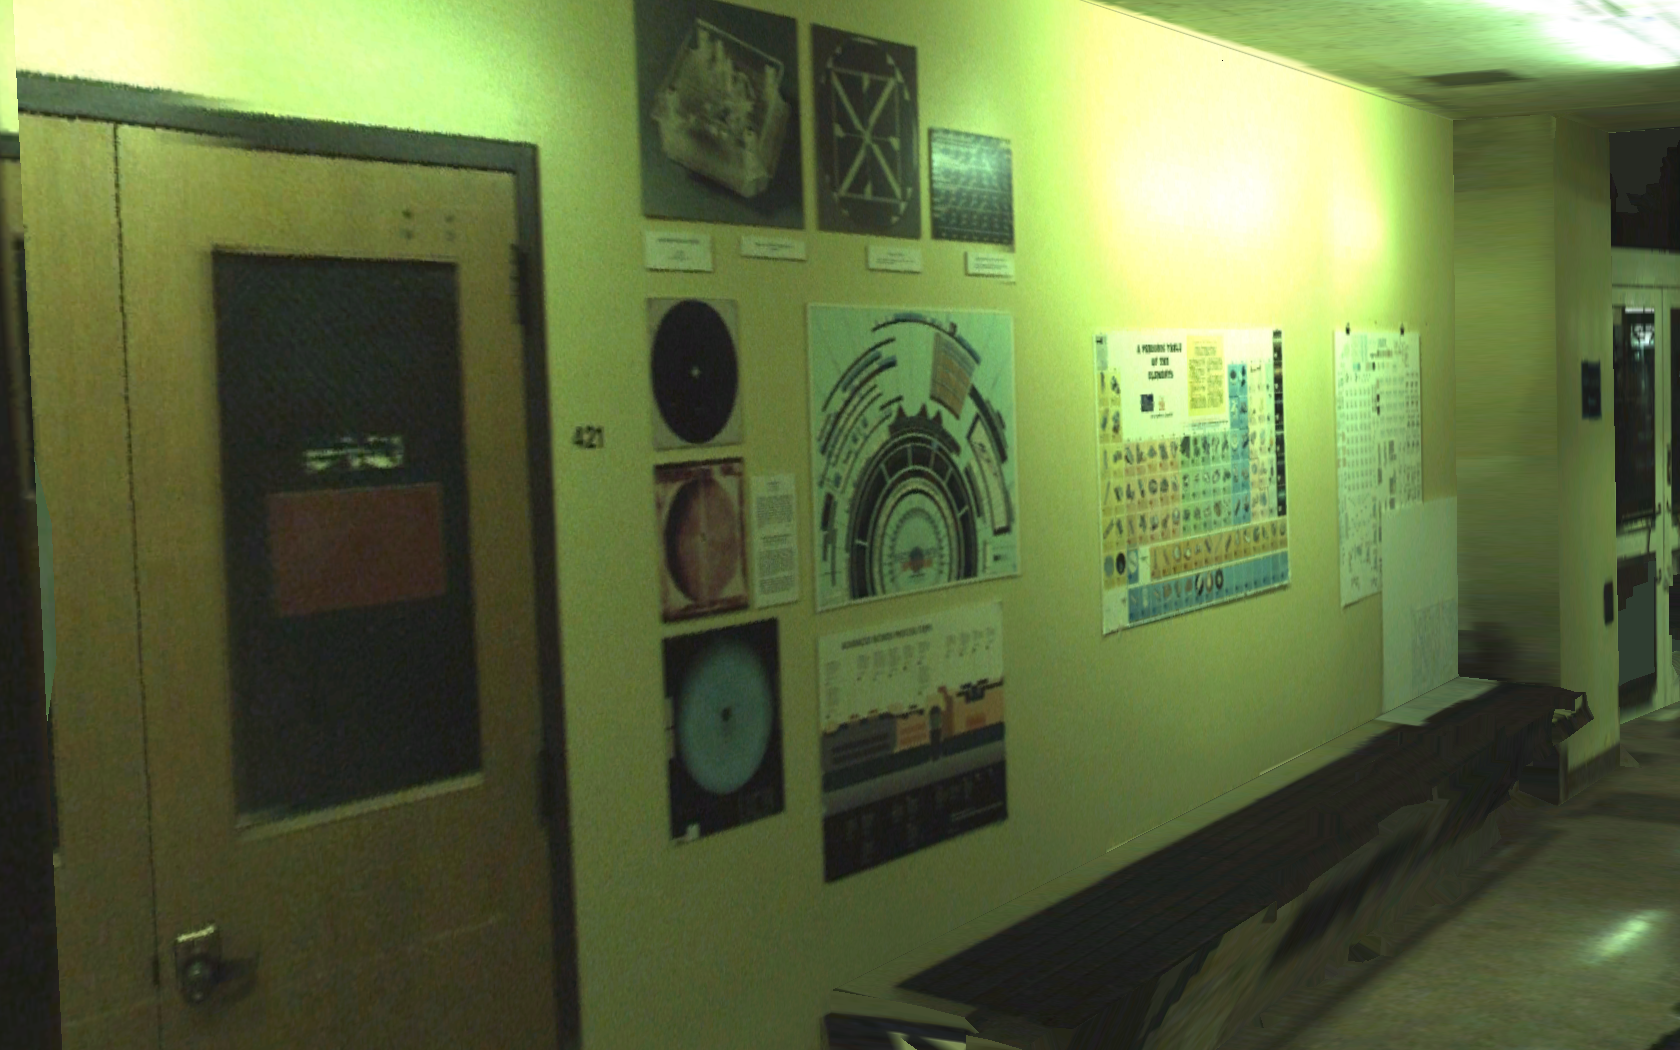
\includegraphics[width=2in]{results_swarm_2_3d.jpg}
  }
  \subfloat[][]{
    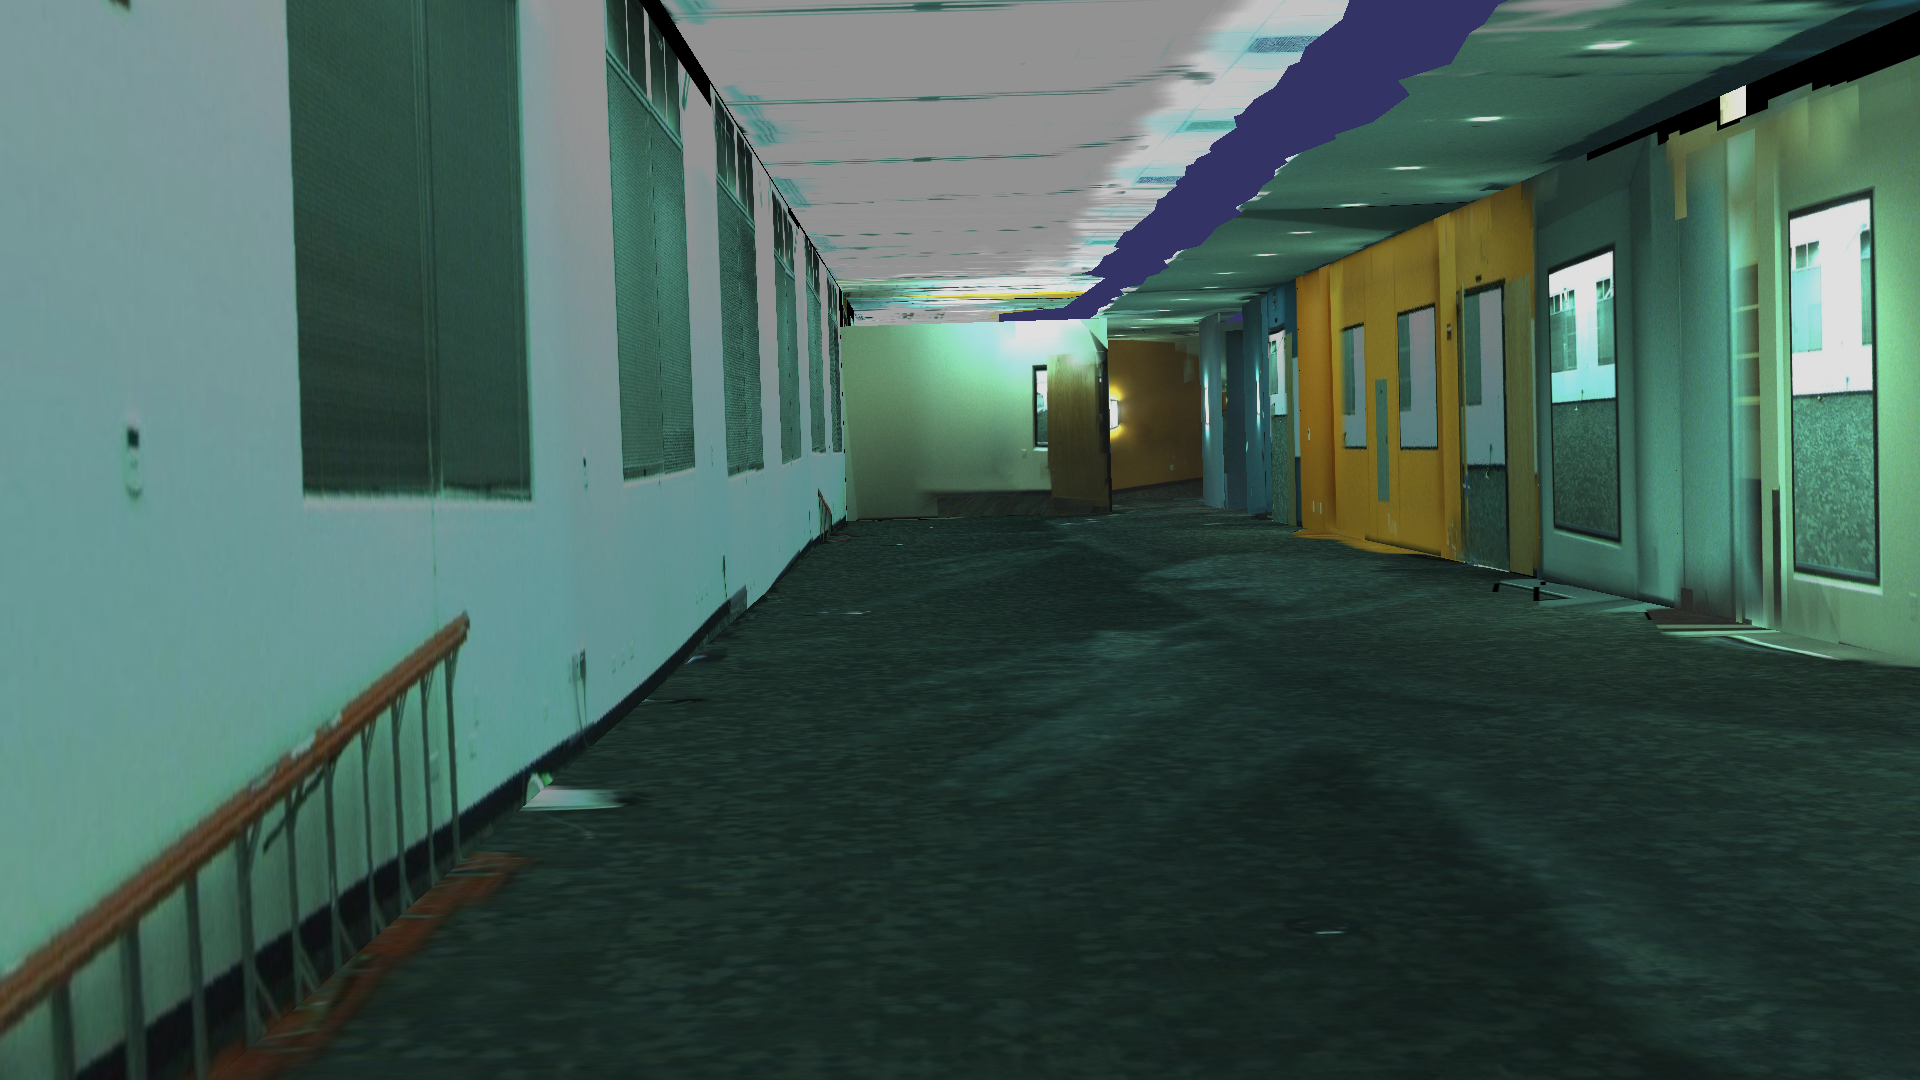
\includegraphics[width=2in]{results_swarm_5_v.jpg}
    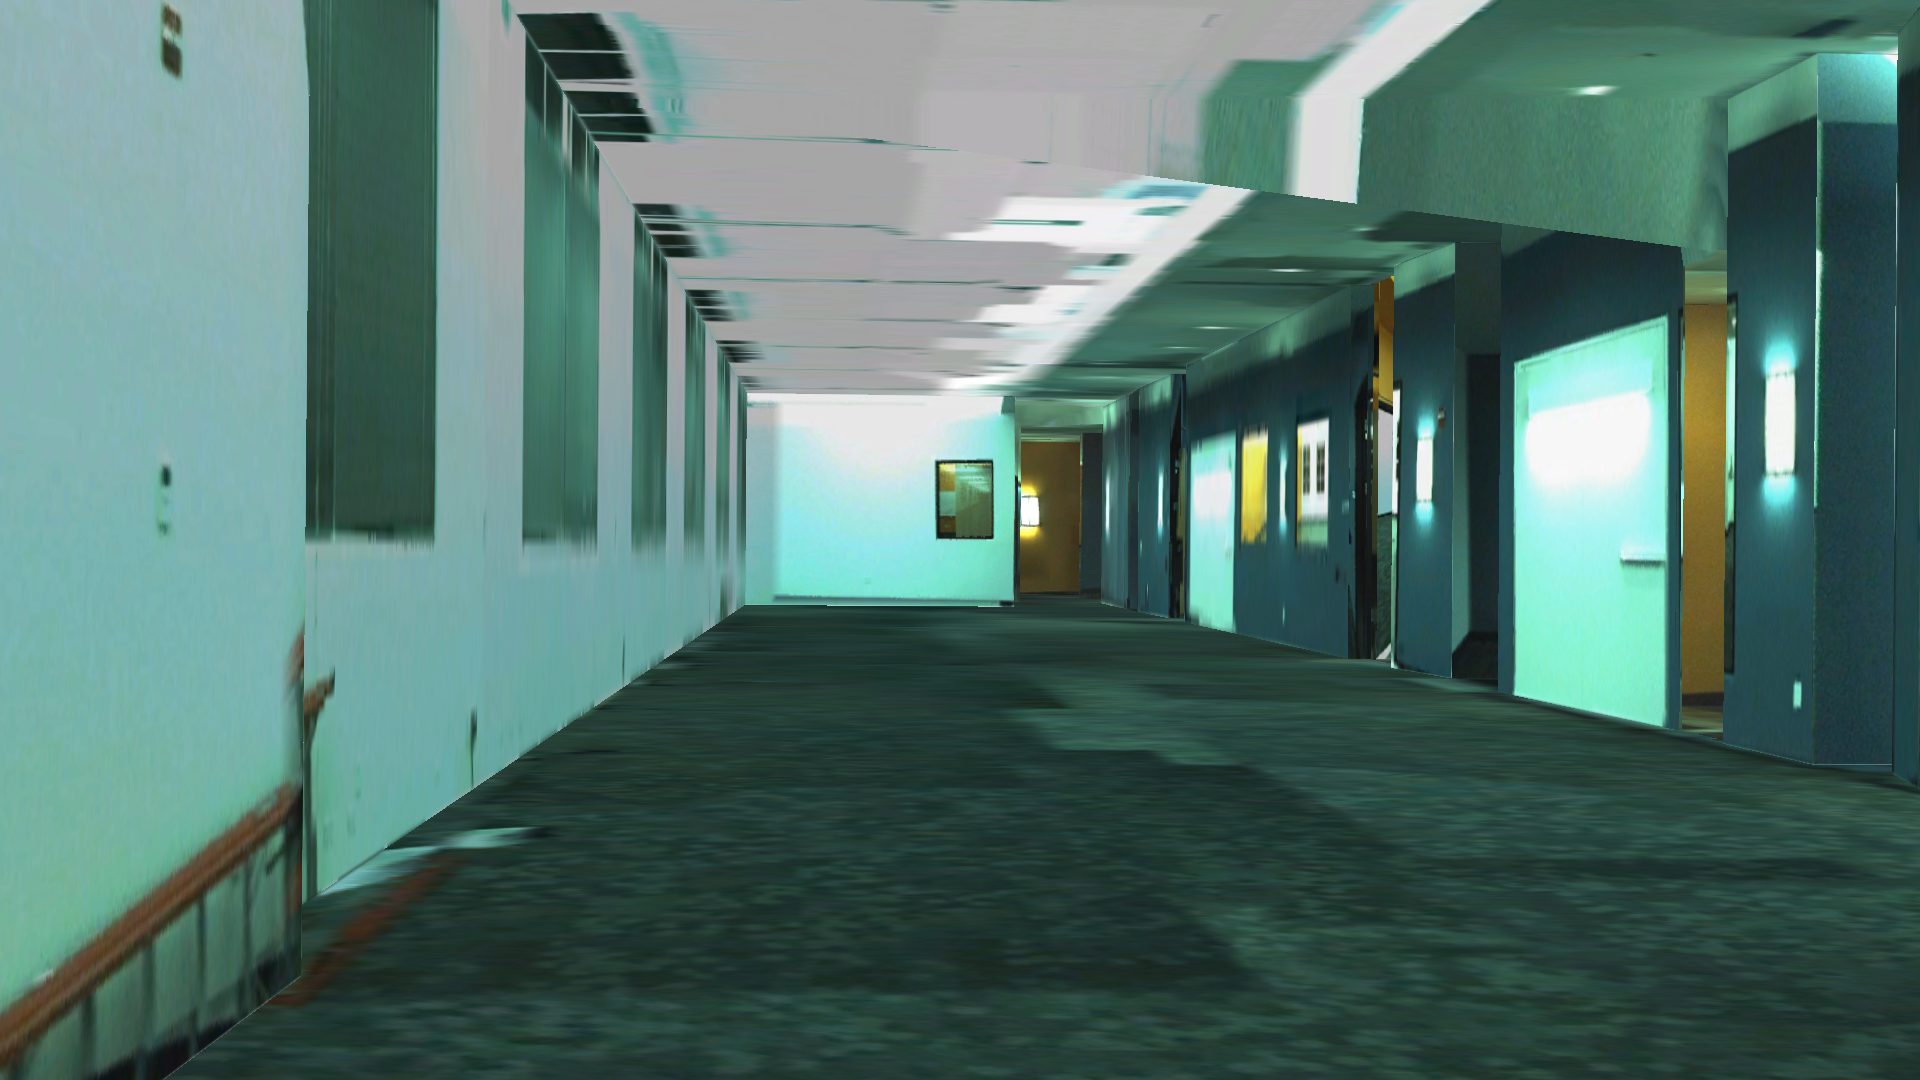
\includegraphics[width=2in]{results_swarm_5_2d.jpg}
    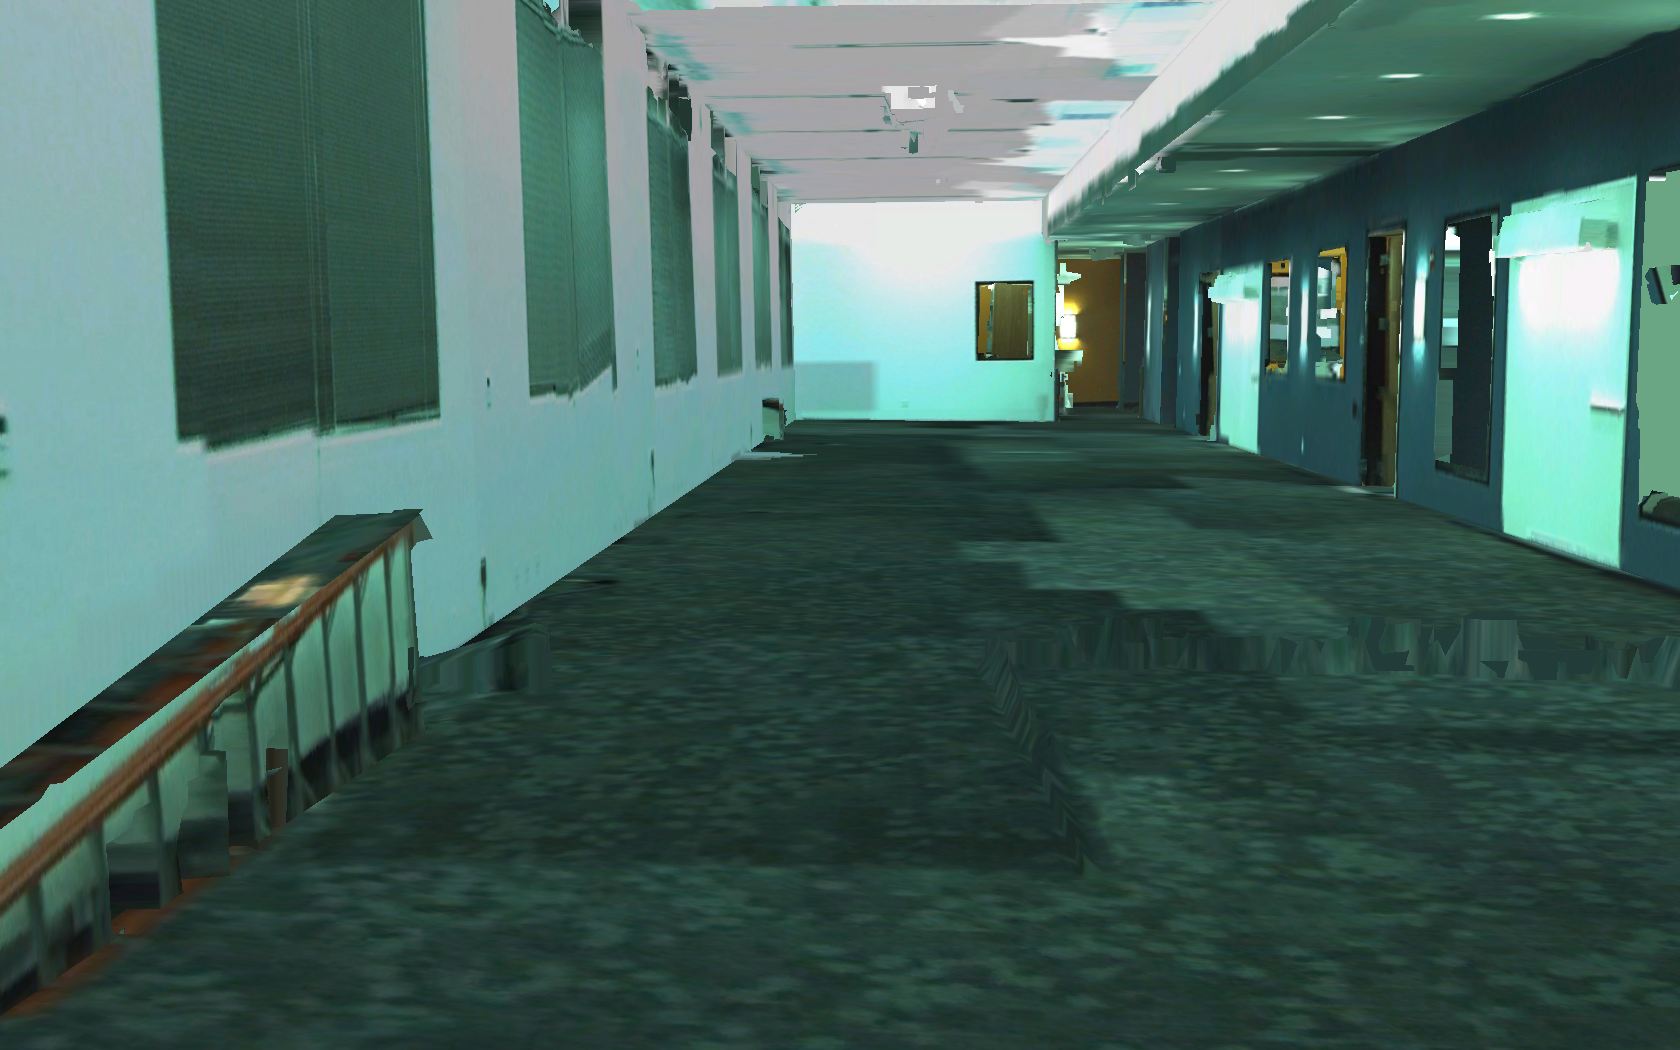
\includegraphics[width=2in]{results_swarm_5_3d.jpg}
  }

  \caption{The same indoor environment, as generated using (a) PCA
    plane-fitting, (b) Floor plan extrusion, (c) Watertight mesh
    generation. The first two are low-resolution models, while the
    third is high-resolution}
  \label{fig:modelcomparisons}
\end{figure}

Our approach was tested with three different geometry-reconstruction
methods, a PCA-based plane-fitting method \cite{sanchez2012point}, a
floor plan extrusion method \cite{turnerfloorplan}, and a
voxel-carving mesh generation method \cite{turnerwatertight}. The
first two methods generate lower-resolution models, containing only
major walls, ceilings and floors. The third method generates
high-resolution models, and attempts to reconstruct all scanned
objects in the environment. A comparison of all three methods as
applied to the same dataset is shown in Figure
\ref{fig:modelcomparisons}

\begin{figure}
  \centering
  \caption{low resolution stuff. (a) is not watertight}
  \label{fig:lowresmodels}
\end{figure}

The PCA and floor plan methods produce models at a similar level of
detail. As visible in Figure \ref{fig:lowresmodels}(a), the PCA method
is not watertight, while the floor plan method is. As a result, the
PCA-generated model contains holes where surfaces were not adequately
scanned. On the other hand, the watertight floor plan model sometimes
must make assumptions about the location of surfaces that were not
adequately scanned, in order to maintain watertightness. Because
buildings generally follow straight lines and right angle corners
however, such assumptions tend to be correct. Additionally, the
floor-plan method is generally superior at reconstructing smaller
surfaces, such as small walls, or to approximate curved surfaces,
while the PCA method only fits large planes, and fails in both
cases. As a result, the floor-plan method usually produces more
visually pleasing low-resolution models, and is the method of choice
for generating textured low-resolution models.

\begin{figure}
  \caption{2d vs 3d}
  \label{fig:2dvs3d}
\end{figure}

High-resolution models, as generated by the voxel-carving method, can
produce more accurate reconstructions of environment geometry. With
such models, region partitioning, as described in Section
\ref{sec:geometryPartitioning}, plays an important factor in the
quality of generated textures. If regions are small, boundaries
between adjacent textures become visible, and since each region is
processed independently, image alignment procedures are performed
across smaller areas. If regions are large, then the difference
between the 3D surface geometry and the approximated 2D texturing
surface become large as well, introducing greater texture projection
error. Additionally, in areas where pose error or surface
reconstruction error is high, 3D objects in images do not get
accurately projected onto their modeled counterparts. While large
objects can be aligned to geometry via the methods in Section
\ref{sec:geometryAlignment}, smaller objects such as plants or
computers are difficult to line up to geometry references. While the
compositing techniques is Section \ref{sec:imageCompositing} can
ensure that textures for small objects appear seamless, such textures
may not map accurately upon their corresponding geometry, leading to
visually obvious discrepancies in the textured model. Figure
\ref{fig:2dvs3d} demonstrates this by showcasing the low-resolution
floor plan approach alongside the high-resolution voxel-carving
approach.

As visible in Figure \ref{fig:2dvs3d} and other images in this
section, 2D models using the floor plan approach are generally
preferred, as they provide enough detail in geometry to reconstruct
the basic layout of an environment, while textures can be used to
visualize smaller details. On the other hand, for applications where
furniture and smaller interior details are important, applying
textures to the 3D voxel-carved models provides useful image-based
context for visualizing indoor areas. Figures 1-3 demonstrate further
interior and exterior views of a number of 2D models, while Figures
4-6 demonstrate interior and exterior views of 3D models.


\message{ !name(masters.tex) !offset(1065) }

\end{document} 
